% Options for packages loaded elsewhere
\PassOptionsToPackage{unicode}{hyperref}
\PassOptionsToPackage{hyphens}{url}
%
\documentclass[
  x11names]{article}
\usepackage{amsmath,amssymb}
\usepackage{lmodern}
\usepackage{iftex}
\ifPDFTeX
  \usepackage[T1]{fontenc}
  \usepackage[utf8]{inputenc}
  \usepackage{textcomp} % provide euro and other symbols
\else % if luatex or xetex
  \usepackage{unicode-math}
  \defaultfontfeatures{Scale=MatchLowercase}
  \defaultfontfeatures[\rmfamily]{Ligatures=TeX,Scale=1}
\fi
% Use upquote if available, for straight quotes in verbatim environments
\IfFileExists{upquote.sty}{\usepackage{upquote}}{}
\IfFileExists{microtype.sty}{% use microtype if available
  \usepackage[]{microtype}
  \UseMicrotypeSet[protrusion]{basicmath} % disable protrusion for tt fonts
}{}
\makeatletter
\@ifundefined{KOMAClassName}{% if non-KOMA class
  \IfFileExists{parskip.sty}{%
    \usepackage{parskip}
  }{% else
    \setlength{\parindent}{0pt}
    \setlength{\parskip}{6pt plus 2pt minus 1pt}}
}{% if KOMA class
  \KOMAoptions{parskip=half}}
\makeatother
\usepackage{xcolor}
\usepackage[margin=1in]{geometry}
\usepackage{graphicx}
\makeatletter
\def\maxwidth{\ifdim\Gin@nat@width>\linewidth\linewidth\else\Gin@nat@width\fi}
\def\maxheight{\ifdim\Gin@nat@height>\textheight\textheight\else\Gin@nat@height\fi}
\makeatother
% Scale images if necessary, so that they will not overflow the page
% margins by default, and it is still possible to overwrite the defaults
% using explicit options in \includegraphics[width, height, ...]{}
\setkeys{Gin}{width=\maxwidth,height=\maxheight,keepaspectratio}
% Set default figure placement to htbp
\makeatletter
\def\fps@figure{htbp}
\makeatother
\setlength{\emergencystretch}{3em} % prevent overfull lines
\providecommand{\tightlist}{%
  \setlength{\itemsep}{0pt}\setlength{\parskip}{0pt}}
\setcounter{secnumdepth}{-\maxdimen} % remove section numbering
\usepackage{fontspec} \usepackage{titling} \pretitle{\begin{center} \vspace{-3cm}
\includegraphics[width=\linewidth]{images/Base_info/logo.png}\LARGE\\} \posttitle{\end{center}} \usepackage{float} \usepackage{fancyhdr} \usepackage{ragged2e} \usepackage{caption} \usepackage{colortbl} \captionsetup[figure]{labelformat=empty} \arrayrulecolor{white} \pagestyle{fancy} \fancyhead[L,C]{} \fancypagestyle{plain}{\pagestyle{fancy}} \PassOptionsToPackage{dvipsnames,svgnames*,x11names*}{xcolor} \definecolor{ceil}{rgb}{0.57, 0.63, 0.81} \usepackage[export]{adjustbox} \usepackage{wrapfig} \usepackage{graphicx} \usepackage{caption}
\usepackage{booktabs}
\usepackage{longtable}
\usepackage{array}
\usepackage{multirow}
\usepackage{wrapfig}
\usepackage{float}
\usepackage{colortbl}
\usepackage{pdflscape}
\usepackage{tabu}
\usepackage{threeparttable}
\usepackage{threeparttablex}
\usepackage[normalem]{ulem}
\usepackage{makecell}
\usepackage{xcolor}
\ifLuaTeX
  \usepackage{selnolig}  % disable illegal ligatures
\fi
\IfFileExists{bookmark.sty}{\usepackage{bookmark}}{\usepackage{hyperref}}
\IfFileExists{xurl.sty}{\usepackage{xurl}}{} % add URL line breaks if available
\urlstyle{same} % disable monospaced font for URLs
\hypersetup{
  hidelinks,
  pdfcreator={LaTeX via pandoc}}

\author{}
\date{\vspace{-2.5em}Fecha de creación: 03 April, 2023}

\begin{document}

\setmainfont{Arial}
\setsansfont{Arial}
\setmonofont{Arial}

\newcommand\invisiblesection[1]{%
  \refstepcounter{section}%
  \addcontentsline{toc}{section}{\protect\numberline{\thesection}#1}%
  \sectionmark{#1}}

\fancyhead[R]{\textbf{http://doi.org/10.31687/SaremLR.19.203}}

%
  \refstepcounter{section}%
  \addcontentsline{toc}{section}{\protect\numberline{\thesection}GENERALIDADES}%
  \sectionmark{GENERALIDADES}
\vspace{-0.4cm}


\includegraphics[width=1\linewidth]{images/Base_info/logo}

\vspace{1cm}

\begin{minipage}{0.7\textwidth}
\vspace{0.3cm}
\fontsize{20}{24}\selectfont\textit{Pecari tajacu}

\vspace{0.3cm}
\fontsize{30}{36}\selectfont Pecarí de collar
\end{minipage}
\hspace{0.05\textwidth}
\begin{minipage}{0.25\textwidth}

\includegraphics[width=\textwidth]{images/vu.png}
\end{minipage}

\normalsize

\begin{figure}[H]

{\centering 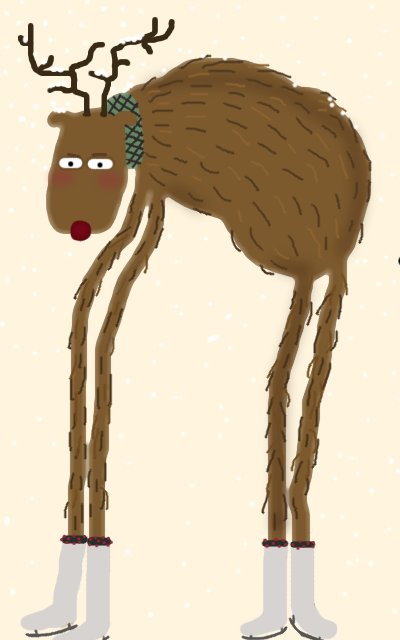
\includegraphics[width=0.35\linewidth]{photos/Blastocerus dichotomus} 

}

\caption{Fotos por Salvador Dali}\label{fig:image}
\end{figure}

\begin{center}\rule{0.5\linewidth}{0.5pt}\end{center}

\justifying

\textbf{Citar como:} Camino, Micaela; Cirignoli, Sebastián; Varela,
Diego; Barri, Fernando; Aprile, Gustavo; Periago, María Eugenia; de
Bustos, Soledad; Quiroga, Verónica A.; Torres, Ricardo M.; Di Martino,
Sebastián. (2019). \emph{Pecari tajacu}. En: SAyDS--SAREM (eds.)
Categorización 2019 de los mamíferos de Argentina según su riesgo de
extinción. Lista Roja de los mamíferos de Argentina.
\url{http://doi.org/10.31687/SaremLR.19.203}

\begin{center}\rule{0.5\linewidth}{0.5pt}\end{center}

\newpage

%
  \refstepcounter{section}%
  \addcontentsline{toc}{section}{\protect\numberline{\thesection}ÁREA DE DISTRIBUCIÓN ACTUAL}%
  \sectionmark{ÁREA DE DISTRIBUCIÓN ACTUAL}
\begin{table}[H]
\centering
\begin{tabular}[t]{>{\raggedright\arraybackslash}m{16cm}>{}m{16cm}}
\toprule
\cellcolor{ceil}{\textcolor{white}{\textbf{\rule{0pt}{14pt}ÁREA DE DISTRIBUCIÓN ACTUAL}}}\\
\bottomrule
\end{tabular}
\end{table}

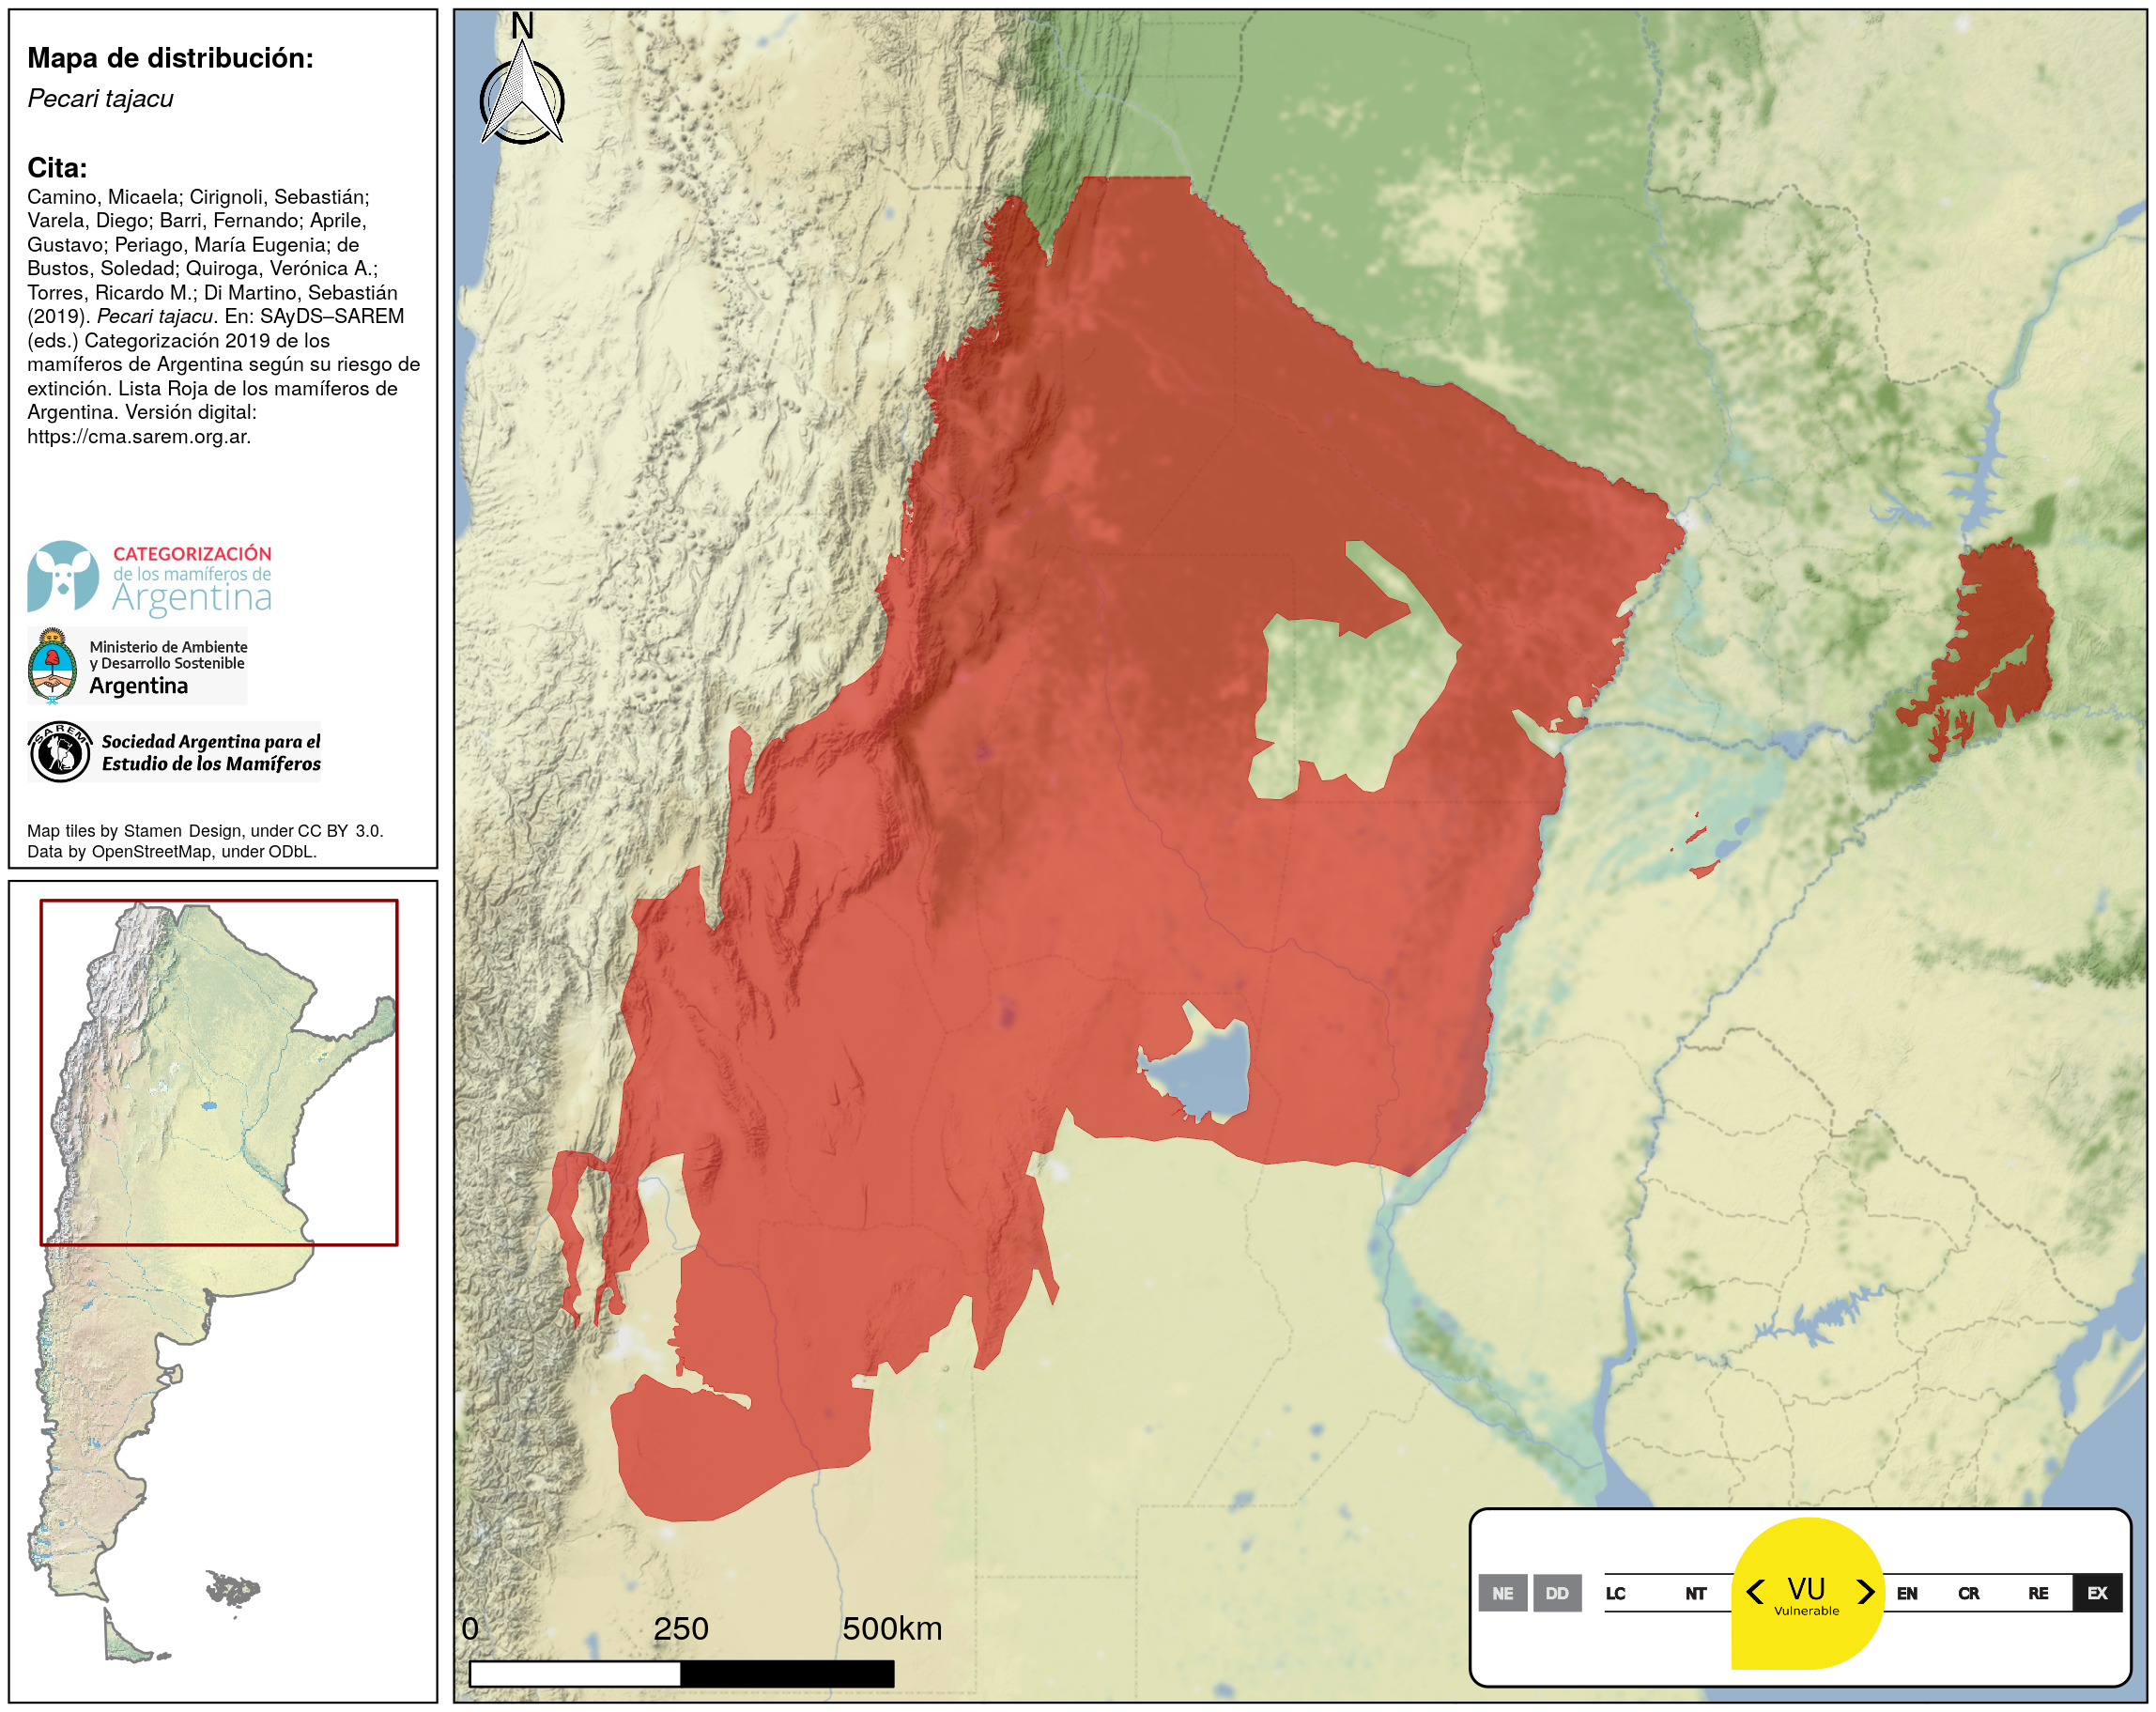
\includegraphics[width=1\linewidth]{maps/Cetartiodactyla/Pecari_tajacu}

%
  \refstepcounter{section}%
  \addcontentsline{toc}{section}{\protect\numberline{\thesection}CATEGORÍAS DE CONSERVACIÓN}%
  \sectionmark{CATEGORÍAS DE CONSERVACIÓN}
\begin{table}[H]
\centering
\begin{tabular}[t]{>{\raggedright\arraybackslash}m{16cm}>{}m{16cm}}
\toprule
\cellcolor{ceil}{\textcolor{white}{\textbf{\rule{0pt}{14pt}CATEGORÍAS DE CONSERVACIÓN}}}\\
\bottomrule
\end{tabular}
\end{table}

\vspace{-0.4cm}

\textbf{Categoría Nacional de Conservación 2019}

VU (Vulnerable)

\textbf{Criterios y subcriterios}

A4cd

\textbf{Justificación de la categorización}

El pecarí de collar está ampliamente distribuido en el centro y norte de
Argentina. Se encuentra en las ecorregiones de Yungas, Chaco Seco, Chaco
Húmedo, Selva Paranaense, y está siendo reintroducido en los Esteros del
Iberá.~Esta especie, respecto de las otras dos de pecaríes, es la menos
susceptible a la degradación del bosque, la fragmentación y a la caza
(Altrichter \& Boaglio, 2004); también presenta una dieta generalista y
su productividad es más alta (Altrichter 2006). Sin embargo, el pecarí
de collar necesita de bosques nativos para persistir (Altrichter \&
Boaglio~2004; Periago et al.~2017). Grandes superficies de bosques
nativos están siendo reemplazadas por otros tipos de cobertura con fines
productivos (Hansen et al.~2013); por lo que la pérdida de bosques
amenaza la conservación de este pecarí. Además, la especie se encuentra
bajo altísima presión de cacería en todo su rango de distribución y está
llevando a la extinción local de la especie en algunas localidades. Se
sospecha e infiere una reducción en el tamaño poblacional superior al
30\% producto de la disminución del área de ocupación (AOO), extensión
de presencia (EOO) y calidad del hábitat, pasada (15 años) y proyectada
(10 años) hacia el futuro. Las causas de la reducción del AOO son: (1)
la transformación completa del hábitat de la especie -principalmente en
Selva Pedemontana de Yungas y en el Chaco Seco y Húmedo-, debido al
avance~ de la producción intensiva agrícola y ganadera; (2) la
persistencia o aumento de los niveles actuales de cacería y (3) otras
amenazas en los fragmentos de hábitat remanentes.

\textbf{Categoría Res. SAyDS 1030/04}

NA (No Amenazada)

\textbf{Categorías nacionales de conservación previas (SAREM)}

\arrayrulecolor{white}

%
  \refstepcounter{section}%
  \addcontentsline{toc}{section}{\protect\numberline{\thesection}TAXONOMÍA Y NOMENCLATURA}%
  \sectionmark{TAXONOMÍA Y NOMENCLATURA}
\begin{table}[H]
\centering
\begin{tabular}[t]{>{\raggedright\arraybackslash}m{16cm}>{}m{16cm}}
\toprule
\cellcolor{ceil}{\textcolor{white}{\textbf{\rule{0pt}{14pt}TAXONOMÍA Y NOMENCLATURA}}}\\
\bottomrule
\end{tabular}
\end{table}

%
  \refstepcounter{section}%
  \addcontentsline{toc}{section}{\protect\numberline{\thesection}INFORMACIÓN RELEVANTE PARA LA EVALUACIÓN}%
  \sectionmark{INFORMACIÓN RELEVANTE PARA LA EVALUACIÓN}
\begin{table}[H]
\centering
\begin{tabular}[t]{>{\raggedright\arraybackslash}m{16cm}>{}m{16cm}}
\toprule
\cellcolor{ceil}{\textcolor{white}{\textbf{\rule{0pt}{14pt}INFORMACIÓN RELEVANTE PARA LA EVALUACIÓN}}}\\
\bottomrule
\end{tabular}
\end{table}

%
  \refstepcounter{section}%
  \addcontentsline{toc}{section}{\protect\numberline{\thesection}RANGO GEOGRÁFICO, OCURRENCIA Y ABUNDANCIA Y NOMENCLATURA}%
  \sectionmark{RANGO GEOGRÁFICO, OCURRENCIA Y ABUNDANCIA Y NOMENCLATURA}
\begin{table}[H]
\centering
\begin{tabular}[t]{>{\raggedright\arraybackslash}m{16cm}>{}m{16cm}}
\toprule
\cellcolor{ceil}{\textcolor{white}{\textbf{\rule{0pt}{14pt}RANGO GEOGRÁFICO, OCURRENCIA Y ABUNDANCIA Y NOMENCLATURA}}}\\
\bottomrule
\end{tabular}
\end{table}

%
  \refstepcounter{section}%
  \addcontentsline{toc}{section}{\protect\numberline{\thesection}DATOS MORFOMÉTRICOS}%
  \sectionmark{DATOS MORFOMÉTRICOS}
\begin{table}[H]
\centering
\begin{tabular}[t]{>{\raggedright\arraybackslash}m{16cm}>{}m{16cm}}
\toprule
\cellcolor{ceil}{\textcolor{white}{\textbf{\rule{0pt}{14pt}DATOS MORFOMÉTRICOS}}}\\
\bottomrule
\end{tabular}
\end{table}

%
  \refstepcounter{section}%
  \addcontentsline{toc}{section}{\protect\numberline{\thesection}RASGOS ETO-ECOLÓGICOS}%
  \sectionmark{RASGOS ETO-ECOLÓGICOS}
\begin{table}[H]
\centering
\begin{tabular}[t]{>{\raggedright\arraybackslash}m{16cm}>{}m{16cm}}
\toprule
\cellcolor{ceil}{\textcolor{white}{\textbf{\rule{0pt}{14pt}RASGOS ETO-ECOLÓGICOS}}}\\
\bottomrule
\end{tabular}
\end{table}

%
  \refstepcounter{section}%
  \addcontentsline{toc}{section}{\protect\numberline{\thesection}CONSERVACIÓN E INVESTIGACIÓN}%
  \sectionmark{CONSERVACIÓN E INVESTIGACIÓN}
\begin{table}[H]
\centering
\begin{tabular}[t]{>{\raggedright\arraybackslash}m{16cm}>{}m{16cm}}
\toprule
\cellcolor{ceil}{\textcolor{white}{\textbf{\rule{0pt}{14pt}CONSERVACIÓN E INVESTIGACIÓN}}}\\
\bottomrule
\end{tabular}
\end{table}

%
  \refstepcounter{section}%
  \addcontentsline{toc}{section}{\protect\numberline{\thesection}BIBLIOGRAFÍA}%
  \sectionmark{BIBLIOGRAFÍA}
\begin{table}[H]
\centering
\begin{tabular}[t]{>{\raggedright\arraybackslash}m{16cm}>{}m{16cm}}
\toprule
\cellcolor{ceil}{\textcolor{white}{\textbf{\rule{0pt}{14pt}BIBLIOGRAFÍA}}}\\
\bottomrule
\end{tabular}
\end{table}

\newpage

%
  \refstepcounter{section}%
  \addcontentsline{toc}{section}{\protect\numberline{\thesection}AUTORES}%
  \sectionmark{AUTORES}
\begin{table}[H]
\centering
\begin{tabular}[t]{>{\raggedright\arraybackslash}m{16cm}>{}m{16cm}}
\toprule
\cellcolor{ceil}{\textcolor{white}{\textbf{\rule{0pt}{14pt}AUTORES}}}\\
\bottomrule
\end{tabular}
\end{table}

\textbf{AUTORES}

\begin{tabu} to \linewidth {>{}l>{\raggedright\arraybackslash}p{2cm}>{\raggedright}X}
\toprule
\textbf{\cellcolor{gray!6}{Aprile, Gustavo}} & \cellcolor{gray!6}{} & \cellcolor{gray!6}{Asociación para la Conservación y Estudio de la Naturaleza (ACEN), Buenos Aires, Argentina}\\
\textbf{Barri, Fernando} &  & Instituto de Diversidad y Ecología Animal (IDEA), CONICET-Universidad Nacional de Córdoba, Córdoba, Argentina\\
\textbf{\cellcolor{gray!6}{Camino, Micaela}} & \cellcolor{gray!6}{} & \cellcolor{gray!6}{Laboratorio de Biología de la Conservación, Centro de Ecología Aplicada del Litoral (CECOAL) - CONICET, Corrientes, Argentina}\\
\textbf{Cirignoli, Sebastián} &  & Centro de Investigaciones del Bosque Atlántico (CeIBA), Puerto Iguazú, Misiones, Argentina\\
\textbf{\cellcolor{gray!6}{de Bustos, Soledad}} & \cellcolor{gray!6}{} & \cellcolor{gray!6}{Secretaría de Ambiente y Desarrollo Sustentable de la Provincia de Salta y Fundación Biodiversidad, Salta, Salta, Argentina}\\
\addlinespace
\textbf{Di Martino, Sebastián} &  & The Conservation Land Trust Argentina (CLT), Mercedes, Corrientes, Argentina\\
\textbf{\cellcolor{gray!6}{Periago, María Eugenia}} & \cellcolor{gray!6}{} & \cellcolor{gray!6}{Fundación Vida Silvestre Argentina (FVSA), Misiones, Argentina}\\
\textbf{Quiroga, Verónica A.} &  & Instituto de Diversidad y Ecología Animal (IDEA - CONICET), Centro de Zoología Aplicada, Universidad Nacional de Córdoba - Centro de Investigaciones del Bosque Atlántico (CeIBA), Córdoba, Argentina\\
\textbf{\cellcolor{gray!6}{Torres, Ricardo M.}} & \cellcolor{gray!6}{} & \cellcolor{gray!6}{Instituto de Diversidad y Ecología Animal (IDEA), CONICET-Universidad Nacional de Córdoba, Córdoba, Argentina}\\
\textbf{Varela, Diego} &  & Instituto de Biología Subtropical (IBS), CONICET-Universidad Nacional de Misiones y Centro de Investigaciones del Bosque Atlántico (CeIBA), Puerto Iguazú, Misiones, Argentina\\
\bottomrule
\end{tabu}

\textbf{COLABORADORES}

\begin{tabu} to \linewidth {>{}l>{\raggedright\arraybackslash}p{2cm}>{\raggedright}X}
\toprule
\textbf{\cellcolor{gray!6}{Albanesi, Sebastián}} & \cellcolor{gray!6}{} & \cellcolor{gray!6}{Instituto de Biodiversidad Neotropical, Universidad Nacional de Tucumán - CONICET, Yerba Buena, Tucumán, Argentina}\\
\textbf{Alderete, Edgar} &  & , , Argentina\\
\textbf{\cellcolor{gray!6}{Alveira, Mariela}} & \cellcolor{gray!6}{} & \cellcolor{gray!6}{Programa SIPAP, Secretaria de Ambiente y Desarrollo Sustentable de Salta, Salta, Argentina}\\
\textbf{Bardavid, Sofía} &  & Instituto de Ecorregiones Andinas (INECOA), Universidad Nacional de Jujuy - CONICET, S.S. de Jujuy, Jujuy, Argentina\\
\textbf{\cellcolor{gray!6}{Borghi, Carlos E.}} & \cellcolor{gray!6}{} & \cellcolor{gray!6}{INTERBIODES (Interacciones Biológicas en el Desierto), CIGEOBIO (CONICET-UNSJ), y Departamento de Biología, FCEFyN, Universidad Nacional de San Juan, San Juan, Argentina}\\
\addlinespace
\textbf{Caruso, María Flavia} &  & Dirección Regional Noroeste-CONICET, Administración de Parques Nacionales y Proyecto Jaguares en el Límite, Salta, Argentina\\
\textbf{\cellcolor{gray!6}{Cuevas, María Fernanda}} & \cellcolor{gray!6}{} & \cellcolor{gray!6}{Grupo de Investigaciones de la Biodiversidad (GiB), Instituto Argentino de Investigaciones de Zonas Aridas (IADIZA), CCT CONICET Mendoza, Mendoza, Argentina}\\
\textbf{de la Colina, Alicia} &  & Fundación Temaikén, Escobar, Buenos Aires, Argentina\\
\textbf{\cellcolor{gray!6}{Gómez, Bibiana}} & \cellcolor{gray!6}{} & \cellcolor{gray!6}{, , Argentina}\\
\textbf{Lartigau, Bernardo} &  & Programa Areas Protegidas, Fundación Vida Silvestre Argentina y Asociación para la Conservación y Estudio de la Naturaleza (ACEN), Buenos Aires, Argentina\\
\addlinespace
\textbf{\cellcolor{gray!6}{Maras, Gustavo A.}} & \cellcolor{gray!6}{} & \cellcolor{gray!6}{Laboratorio de Ecología Aplicada a la Conservación (LEAC), Facultad de Ciencias Naturales, Universidad Nacional de Salta - CONICET, Salta, Salta, Argentina}\\
\textbf{Pautasso, Andres} &  & Museo Provincial de Ciencias Naturales Florentino Ameghino, Santa Fe, Santa Fe, Argentina\\
\textbf{\cellcolor{gray!6}{Perovic, Pablo G.}} & \cellcolor{gray!6}{} & \cellcolor{gray!6}{Dirección Regional Noroeste, Administración de Parques Nacionales y Proyecto Jaguares en el Límite, Salta, Argentina}\\
\textbf{Politi, Natalia} &  & Instituto de Ecorregiones Andinas (INECOA), Universidad Nacional de Jujuy - CONICET - Fundacion CEBio, Jujuy, Argentina\\
\textbf{\cellcolor{gray!6}{Puechagut, Patricia}} & \cellcolor{gray!6}{} & \cellcolor{gray!6}{Universidad Nacional de Jujuy - CONICET y Fundación CEBio, Jujuy, Argentina}\\
\addlinespace
\textbf{Reppucci, Juan I.} &  & CONICET, Administración de Parques Nacionales, Dirección Regional Noroeste y Proyecto Jaguares en el Límite, Salta, Argentina\\
\textbf{\cellcolor{gray!6}{Rivera, Luis O.}} & \cellcolor{gray!6}{} & \cellcolor{gray!6}{Instituto de Ecorregiones Andinas (INECOA), Universidad Nacional de Jujuy - CONICET - Fundacion CEBio, Jujuy, Argentina}\\
\bottomrule
\end{tabu}

\end{document}
